%BEGIN: Tatus
\section{A Testbed for Evaluating Human Interaction with Ubiquitous Computing Environments}\label{sec:tatus}

TATUS \cite{o2005testbed} is as a ubiquitous computing simulator aimed at overcoming the challenges of effectively evaluating human interaction with adaptive ubiquitous technologies. These challenges are mainly imposed by the cost and logistics of building and controlling the context in such real-life environments. In other words, TATUS is a simulator supporting research and development of adaptive software controlling ubiquitous computing environments.\\

Figure \ref{fig:tatus_overview} depicts the high-level overview of the simulator. We can identify two main components: the 3D Simulated Ubiquitous Computing Environment and the System Under Test (SUT).\\

\begin{figure}[H]
	\centering
	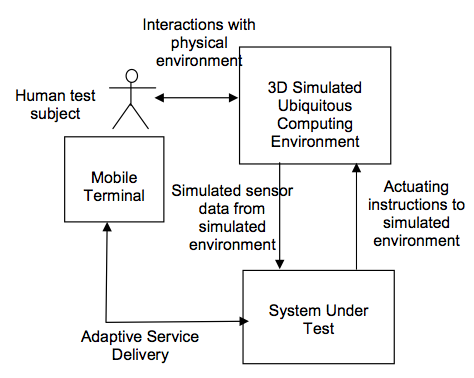
\includegraphics[width=\linewidth]{gfx/Chapter2/tatus_system_overview}
	\caption{High-level simulator overview}
	\label{fig:tatus_overview}
\end{figure}

The 3D simulator was implemented on top of the Half-Life\footnote{\url{http://www.valvesoftware.com}} Game Engine's software development kit (SDK), written in C/C++. Half-Life is a 3D first-person-shooter network game. It is implemented based on client-server architecture with multi-player capabilities (up to 32 players simultaneously). Choosing this game engine was meant to provide a realistic user experience.\\

\begin{figure}[H]
	\centering
	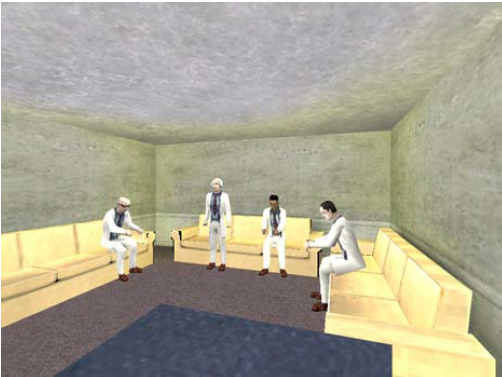
\includegraphics[width=\linewidth]{gfx/Chapter2/tatus_simulated_meeting_room}
	\caption{Simulated meeting room with multiple characters}
	\label{fig:tatus_simulated_meeting_room}
\end{figure}

The actual simulated environment is created using a map editor from Valve called Hammer (a drawing tool for building maps). This can be used to generate complex and realistic environments as the tool offers a wide range of graphical editing possibilities, as exemplified in Figure \ref{fig:tatus_simulated_meeting_room}. The SDK is then able to load a simulated environment's physical settings from the files generated by the map editor.\\

To simulated sensors and actuators they have exploited a concept called \emph{Triggers} from the SDK. They are used to generate associated events based on a player's movements and location. The state of these triggers together with the agents location at a certain point in time represent the state of the simulated environment. To allow easy access to the data, the simulator exposes an API which offers both querying and modifying capabilities. Queries allow to select certain aspects of the current state based on various parameters, whereas through modifications the SUT can impose changes on the simulated environment.\\

A SUT is written as independent pieces of software. It can even run on a separate machines, while multiple SUTs can connect simultaneously to the same simulator. To allow SUTs to run on separate machines the simulator has embedded networking capabilities and communicates through messages. Outgoing messages carry state information, while incoming messages carry instructions to modify the simulated environment. Moreover, to abstract out the network interaction from the SUTs, the simulator provides a Proxy making the communication from the test software's side really easy.\\

As the simulator was developed on top of 3D game engine, it empowers the agent to freely walk around the simulated environment. The interaction between the agent and the based on proximity only. This means that entities will take a specific action when the agent is detected nearby; ''when a player enters a region of a map occupied by a trigger
the associated event is activated e.g. a door is opened'' \cite{o2005testbed}. These triggers can be attached to both physical objects and devices, enabling both categories of objects to be interacted with.\\

The framework exposes an API so that third party software can easily access and modify the context data within the ongoing simulation.
%END: Tatus